\documentclass[conference]{IEEEtran}
\usepackage[T1]{fontenc}
\usepackage{amsmath,amssymb,graphicx,booktabs,url}
\usepackage[hidelinks]{hyperref}
\hypersetup{pdftitle={Laguerre and Full-Input Linearized MPC for RC-Car Simulation: A Progress Report},
pdfauthor={arch1703},pdfsubject={Simulation-only project technical progress report}}

\title{Laguerre and Full-Input Linearized MPC for RC-Car Simulation:
A Progress Report}
\author{\IEEEauthorblockN{arch1703}
\IEEEauthorblockA{Project maintainer\\
Technical progress report --- 28 October 2026\\
\url{https://github.com/arch1703/Laguerre_MPC_Car}}}

\begin{document}
\maketitle

\begin{abstract}
This report documents an autonomous RC-car simulation using Laguerre-parameterized
successively linearized model predictive control (MPC), compared with a
full-input linearized controller. The implementation combines local paired
track-marking measurements, obstacle-aware planning, constrained optimization,
nonlinear validation, and checked stopping. Independently generated obstacles
are observed through a sensor interface; their future trajectories are not
supplied to control. A current deterministic robustness matrix contains sixteen
scenarios evaluated with both controllers, including sensor noise, latency,
losses, uncertain motion classes, limited plant mismatch, and crossing objects.
Both controllers satisfy mission criteria in nine of sixteen cases; all
executed portions satisfy the monitored safety criteria, with no contacts or
road departures. Laguerre reduces the decision count from twelve to eight, but
the mean of per-run called-optimizer medians is 9.03 ms versus 4.63 ms for
full-input MPC. Several uncertainty cases still stall, require fallback, or
lose a verified control. An earlier, separate 23-case controlled study and
selected videos provide developmental context. The evidence supports a
reproducible educational comparison, not universal avoidance, recursive
feasibility, hard-real-time performance, or hardware readiness.
\end{abstract}

\begin{IEEEkeywords}
model predictive control, Laguerre functions, autonomous vehicle simulation,
successive linearization, obstacle avoidance, reproducibility
\end{IEEEkeywords}

\section{Introduction}
Model predictive control repeatedly optimizes a finite sequence of inputs
subject to a model and constraints. It does not require a trained driving
policy. Laguerre functions provide a compact parameterization of the input
sequence, potentially reducing optimization dimension \cite{wang}. However,
dimension reduction alone does not establish a runtime advantage, and
constrained MPC guarantees require assumptions beyond a successful simulation
\cite{mayne}.

The project's purpose is an inspectable demonstration of Laguerre MPC for an
RC-scale vehicle, with ordinary full-input linearized MPC as a matched baseline.
The development progressed from oval tracking to static avoidance, independent
random appearances/disappearances, moving objects, and local-marking following
on multiple tracks. A full nonlinear optimizer is retained as an
obstacle-free tracking baseline; it is not the controller responsible for the
successful moving-obstacle demonstrations.

This report contributes an implementation and evidence snapshot rather than
a new stability theorem. It describes the measurement boundary, failure
semantics, matched comparisons, observed timing, retained negative results,
and planned corrective work. Development is paused for publication.
This document uses an IEEE-conference-style layout but is an unsubmitted,
non-peer-reviewed project report; no IEEE endorsement is implied.

\section{Vehicle and Control Formulation}
\subsection{Discrete Kinematic Model}
The rear-axle state and control are
$x=[X,Y,\psi,v]^\top$ and $u=[\delta,a]^\top$. With sample period $T$,
wheelbase $L$, and explicit Euler integration,
\begin{equation}
x_{k+1}=f(x_k,u_k)=
\begin{bmatrix}
X_k+Tv_k\cos\psi_k\\
Y_k+Tv_k\sin\psi_k\\
\psi_k+T(v_k/L)\tan\delta_k\\
v_k+Ta_k
\end{bmatrix}.
\label{eq:model}
\end{equation}
Plant speed is not clipped to conceal prediction error. The model omits tire
slip, friction limits beyond a reference curvature-speed heuristic, and
real actuator dynamics.

The body extends 0.29 m forward and 0.06 m rearward from the rear axle, with
half-width 0.075 m. A conservative enclosing circle has offset
$b=(0.29-0.06)/2=0.115$ m and radius
$r_b=\sqrt{0.175^2+0.075^2}\simeq0.1904$ m.
Rectangle clearance is logged separately. Required conservative obstacle and
road clearance is 0.05 m.

\begin{table}[t]
\caption{Shared Current Boundary-Experiment Settings}
\label{tab:settings}
\centering
\begin{tabular}{ll}
\toprule
Quantity & Value\\
\midrule
Sample period / target speed & 0.05 s / 0.8 m/s\\
Wheelbase / road half-width & 0.25 m / 0.85 m\\
Prediction / control horizon & 12 / 6 samples\\
Steering magnitude / rate & $22^\circ$ / $120^\circ$/s\\
Acceleration range & $[-4,\;6.67]$ m/s$^2$\\
Jerk magnitude / speed range & 12 m/s$^3$ / $[0,\;3]$ m/s\\
Laguerre modes per input / decay & 4 / 0.7\\
QP iteration cap & 100\\
Guarded linearization passes & Up to 6\\
\bottomrule
\end{tabular}
\end{table}

\subsection{Successively Linearized MPC}
The controller linearizes \eqref{eq:model} along a nonlinear warm rollout:
\begin{equation}
x_{i+1}\simeq A_i x_i+B_i u_i+c_i,\qquad
c_i=f(\bar{x}_i,\bar{u}_i)-A_i\bar{x}_i-B_i\bar{u}_i.
\end{equation}
Lifted prediction matrices form a quadratic tracking objective with input-rate
penalties. Position, heading and speed references follow path arc length;
heading differences are wrapped consistently. Full-input MPC optimizes the
two inputs at each of six control stations, giving twelve variables.
Input, rate, speed, road and separating obstacle constraints are imposed.

The guarded solver limits each relinearization update to 0.12 rad steering
and 1 m/s$^2$ acceleration. Nonlinear versus affine prediction discrepancy
must remain within 0.015 m position and 0.03 rad heading. A failed optimizer
or inaccurate prediction is rejected; these guards do not prove global
convergence or recursive feasibility.

\subsection{Laguerre Input-Increment Parameterization}
For decay $\alpha\in(0,1)$, the first discrete Laguerre function is
$\ell_1(i)=\sqrt{1-\alpha^2}\alpha^i$, $i\geq0$. The implementation uses
\begin{align}
\ell_j(0)&=(-\alpha)^{j-1}\sqrt{1-\alpha^2},\\
\ell_j(i)&=\alpha\ell_j(i-1)+\ell_{j-1}(i-1)-\alpha\ell_{j-1}(i).
\end{align}
For each input channel, increments and absolute inputs satisfy
\begin{equation}
\Delta u_i=\sum_{j=1}^{n_\ell}\ell_j(i)\eta_j,\qquad
u_i=u_{k-1}+\sum_{q=0}^{i}\Delta u_q.
\end{equation}
Four modes per input give eight coefficients in the current comparison.
The truncated finite-horizon basis is not assumed to be exactly orthonormal.
The same costs and physical limits are applied after mapping coefficients
to absolute inputs. Thus the comparison is of parameterizations, not
different vehicle geometry or relaxed constraints.

\section{Sensing, Planning, and Stopping}
\subsection{World--Observation Separation}
A private world generates obstacle motion independently of the vehicle's
control, path, feasibility and outcome. In the random-static mode, births,
positions and optional lifetimes are sampled independently; the first
recordings use fresh, unselected seeds. Arbitrary unsafe appearances are not
postponed to obtain a successful video.

Boundary experiments use independently specified crossing motion: two
transverse sinusoidal movers, one static object and one temporary static
object. The base crossing period is 28 s with amplitude 1.3 m and maximum
speed approximately 0.292 m/s. These are world dynamics, not a directional
forecast delivered to MPC.

The sensor supplies timestamped object IDs, positions, radii, position-error
bounds and admissible motion-speed bounds. It also supplies local paired
boundary lines over an ideal 3.5 m range. Pose and marking association are
assumed known. These are simulated measurements, not camera-derived detections.
Only initialization, sensing and an independent physical monitor access
world truth.

\subsection{Local Track and Obstacle Handling}
The sensed paired boundaries form an open local corridor. The planner tests
center, left and right smooth detours for curvature and footprint clearance.
Global track geometry is not passed to planning as a substitute for missing
measurements. Oval, kidney and chicane tracks use the same controller settings.

For measured obstacle $j$, the controller uses a direction-free inflated
radius of the form
\begin{equation}
R_j^{\rm guard}=R_j+\epsilon_j+m+
\bar{v}_j(\tau_j+H),
\label{eq:inflation}
\end{equation}
where $\epsilon_j$ bounds position error, $m$ is an optional margin,
$\bar{v}_j$ is an admissible speed, $\tau_j$ is measurement age and $H$
includes the relevant prediction or braking horizon and sample allowance.
This is a reachable-region bound, not a velocity or route prediction.
Unknown classes receive the movable-object bound even when physically static.

The sensor uses exactly twenty indexed random draws per acquisition tick,
independent of the number of detected objects or past vehicle trajectory.
Line error is a bounded per-frame coordinate translation, not independent
point jitter; the corridor is shrunk by the stated bound and margin.
Acquisition-frame latency preserves capture times, and the initial frame
bootstraps the stream. Lost markings retain their last observed geometry.

\subsection{Validation and Failure Semantics}
Candidate controls undergo nonlinear rollout checks. A tracking action also
requires a checked braking reserve from its next nominal state. The braking
horizon is twenty-four samples, with terminal speed and acceleration
conditions. The vehicle completes stopping before resuming tracking.
Physical monitoring samples vehicle and world motion separately, including
inter-sample allowances; future truth samples are not used to select commands.

With complete miss-free scans, an absent object is outside the acquired
sensor footprint. It can be excluded from a local stopping tube only after
checking that tube remains inside the observed region as it shrinks with
measurement age and admissible object motion. This does not protect against
arbitrary new objects spawning inside that region.

With Bernoulli missed detections, complete-scan exclusion is disabled.
Repeated negative observations can clear memory only under the configured
containment/confirmation rule, but consecutive misses can still constitute
false absence evidence. No deterministic avoidance guarantee follows.

If no checked action exists, the simulation reports
\texttt{no\_verified\_control} without advancing under an unchecked command.
A stopped car is not automatically successful: stopping below 0.05 m/s for
twelve seconds causes \texttt{stalled}. Current mission success requires
completion, safety margins, zero fallback, and progress of at least
35\% of nominal distance over the \emph{requested} duration.
Safety pass describes only the executed portion.

\section{Experimental Protocol}
\subsection{Two Distinct Evidence Sets}
The earlier controlled study contains twenty-three tracking, static,
appearing/replayed and parameter-sweep cases. Defaults include a 1.2 m/s
target and horizons 20/10; the short-horizon static variant uses 10/5.
Its results are retained separately with an implementation snapshot.
They must not be pooled with the newer boundary robustness matrix.

The current matrix pairs Laguerre and full-input MPC across sixteen
predeclared scenarios, requesting forty seconds per run. Settings are in
Table~\ref{tab:settings}. Each pair shares world configuration, seed 41,
initial state, costs, bounds and indexed disturbances. Observations may differ
because trajectories and sensor footprints differ. Controller order alternates.
Warm-up wall time is recorded separately; all in-run outliers remain included.
One seed per configuration does not estimate a statistical success probability.

\subsection{Metrics and Timing}
Planned-path RMS is distance to the contemporaneous local planned route;
track cross-track error is measured independently against the centerline.
Obstacle detours intentionally increase centerline deviation.

Called-optimizer medians are computed only where MPC was actually invoked,
excluding waiting ticks. The reported aggregate is the arithmetic mean of
sixteen per-run medians, not a pooled tick median. Original all-tick solve-stage
statistics are retained separately. Online time includes sensing, planning,
solve and validation; full-loop time also includes physical monitoring and
simulator bookkeeping. Stage percentiles are not additive.

The optional deadline watchdog selects checked braking if pre-application
elapsed work already exceeds 50 ms. It cannot undo elapsed delay, and
braking computation can itself overrun. Desktop measurements and iteration
caps do not provide hard-real-time guarantees.

\section{Results}
\subsection{Earlier Controlled Study}
All twenty-three cases met that study's safety/completion criteria without
sampled collisions or fallback; accuracy and timing targets were not universally
met. Selected values appear in Table~\ref{tab:earlier}.

\begin{table}[t]
\caption{Earlier Controlled Study: Selected, Separate Results}
\label{tab:earlier}
\centering
\footnotesize
\setlength{\tabcolsep}{4pt}
\begin{tabular}{lrrr}
\toprule
Case & RMS [cm] & Solve [ms] & Step p99 [ms]\\
\midrule
Laguerre tracking & 0.130 & 12.78 & 43.84\\
Full-input tracking & 0.142 & 8.29 & 24.58\\
Nonlinear tracking & 0.142 & 836.54 & 925.97\\
Laguerre static & 0.228 & 28.53 & 56.27\\
Full-input static & 0.249 & 13.77 & 29.24\\
Short-horizon Laguerre static & 0.227 & 10.76 & 24.08\\
\bottomrule
\end{tabular}
\end{table}

Nonlinear tracking missed all 300 deadlines in its fifteen-second experiment.
It is an offline baseline, not evidence of real-time nonlinear obstacle
avoidance. Reduced Laguerre dimension did not produce faster solves than
full-input MPC in the measured small-QP cases.

\subsection{Current Robustness Matrix}
Both controllers pass nine of sixteen missions, with identical pass/fail
patterns. All thirty-two executed portions satisfy monitored safety criteria,
with no contacts or road departures. Table~\ref{tab:current} summarizes
aggregate results; Table~\ref{tab:cases} retains failed conditions.

\begin{table}[t]
\caption{Current Paired Robustness Results}
\label{tab:current}
\centering
\begin{tabular}{lrr}
\toprule
Measurement & Laguerre & Full-input\\
\midrule
Mission pass & 9/16 & 9/16\\
Executed-portion safety pass & 16/16 & 16/16\\
Decision variables & 8 & 12\\
Mean called-solve median [ms] & 9.03 & 4.63\\
Online misses / ticks & 53/11887 & 1/11886\\
Full-loop misses / ticks & 213/11887 & 3/11886\\
\bottomrule
\end{tabular}
\end{table}

\begin{table}[t]
\caption{All Sixteen Conditions: Outcome Shared by Both Controllers}
\label{tab:cases}
\centering
\begin{tabular}{ll}
\toprule
Condition & Mission outcome\\
\midrule
Nominal chicane, kidney, oval & Pass (3 conditions)\\
Bounded marking/object noise & Pass\\
Three-sample acquisition latency & Fail: fallback\\
Brief marking loss & Pass\\
Long marking loss & Fail: stalled\\
Missed detections & Fail: no verified control\\
Unknown motion classes & Fail: stalled\\
Tested plant mismatch & Pass\\
Faster crossings & Fail: rejection/stalled\\
Reversed crossings & Pass\\
Different initial station & Pass\\
Larger objects & Fail: fallback\\
Combined uncertainty & Fail: no verified control\\
Watchdog enabled & Pass; no intervention\\
\bottomrule
\end{tabular}
\end{table}

\begin{figure*}[t]
\centering
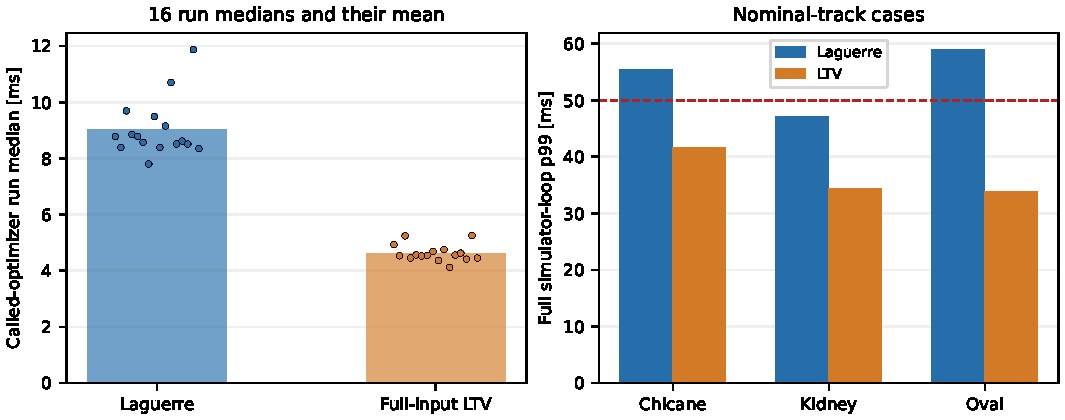
\includegraphics[width=0.95\textwidth]{../assets/comparison.pdf}
\caption{Figures rebuilt from committed CSVs. Left: sixteen called-optimizer
run medians per controller (points) and their arithmetic mean (bars).
Right: full-loop p99 for the three nominal track cases; dashed line denotes
the 50 ms sample budget. Fewer decision variables did not imply lower runtime.}
\label{fig:timing}
\end{figure*}

The nominal kidney pair completes approximately 1.13 laps in forty seconds.
Minimum conservative obstacle clearance is 11.88 cm for both. Planned-path
RMS is 2.71 cm for Laguerre and 2.70 cm for full-input MPC; full-loop p99 is
47.16 and 34.38 ms respectively. These percentiles do not imply zero outliers.

Latency causes 77 rejected QPs/fallbacks per controller; larger objects cause
one each. Faster crossings cause 237 rejected QPs each and then a stall.
An exit flag of $-2$ establishes optimizer rejection, not physical
unavoidability. Compatibility of the geometric planner, finite-horizon QP
and restarting state remains a working diagnosis.

The missed-detection Laguerre run ends at 35.00 s with relevant object age
17.75 s; combined uncertainty ends at 39.65 s with age 19.40 s.
Growing stale reachable regions require investigation, not silent deletion.
Unknown-class conservatism can legitimately block passage.
Long marking loss ends in a stall before markings return. The watchdog
pair records zero interventions and therefore does not exercise actual
overrun recovery.

\subsection{Selected Recordings}
The latest noisy-sensing chicane recording completes forty seconds and
1.025 laps, with 3.92 cm path RMS, 15.11 cm minimum conservative clearance,
and no contacts or fallback. It uses the first predeclared noisy case, not
a favorable seed retry. Figure~\ref{fig:video} shows a recorded frame.
Control runs at 20 Hz; the H.264 recording contains 400 frames at 10 fps.

\begin{figure*}[t]
\centering
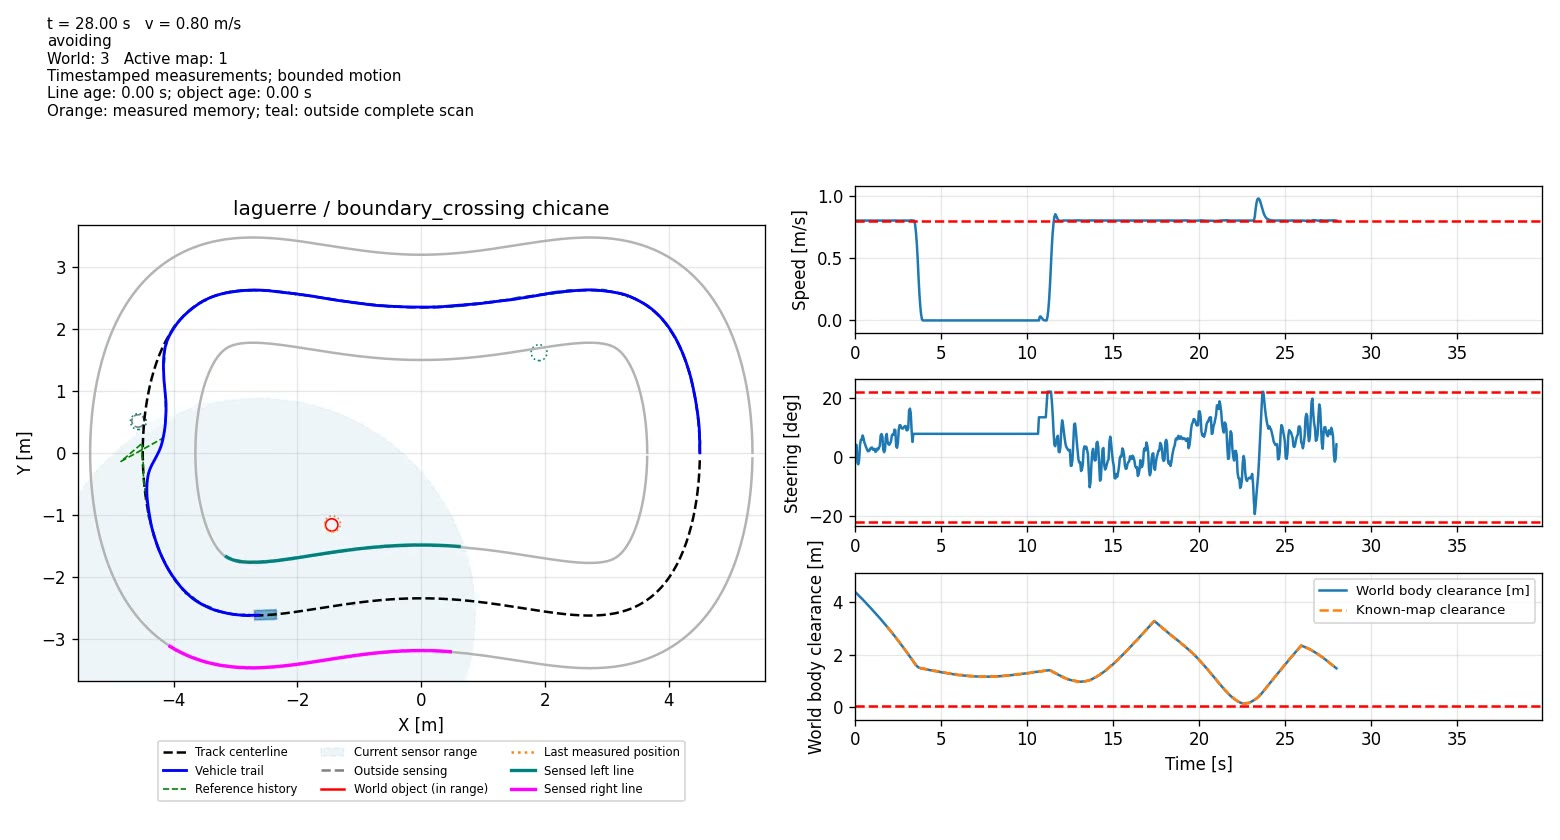
\includegraphics[width=0.90\textwidth]{../assets/noisy_chicane.jpg}
\caption{Recorded noisy-sensing Laguerre simulation, not an illustrative
rendering of a hypothetical outcome. Physical truth, measured memory, local
markings, speed, steering and clearance are displayed separately. The README
links directly to this video and the advanced cross-track recordings.}
\label{fig:video}
\end{figure*}

Earlier cross-track chicane/kidney recordings demonstrate verified
yielding/resumption with a previous implementation. Independent random-static
seed 312882142 completes forty-five seconds without contact/fallback.
The transient-object seed 273210986 is deliberately retained as a failure:
seventeen births and twelve removals occur before a requested sixty-second
run stops at 31.85 s on \texttt{unsafe\_spawn}, without confirmed contact.
That simulator halt is neither a completed mission nor demonstrated physical
emergency braking. Videos and configurations from different stages are not
interchangeable evidence.

\section{Reproducibility and Limitations}
The public repository includes the current MATLAB/Python implementation,
tests, all thirty-two current run CSV sets and manifests, case definitions,
warm-up data, comparisons, checksums, paper source and selected MP4s.
Private local paths are replaced by portable relative run paths, with
original run IDs retained. Duplicate current source snapshots and MAT binaries
are omitted. CSV animation remains supported; MATLAB's saved-bundle replay
API requires an original \texttt{run.mat} or a newly saved simulation.
The earlier study has a separate summary and implementation snapshot.

The controller snapshot passed 51 MATLAB regressions with zero Code Analyzer
messages. Publication changes pass thirteen Python tests, including actual
headless animation exports, portable paths and non-destructive curation.
A prior audit checked 23,773 ticks, 81,099 world rows, 47,006 memory rows and
1,016,888 line pairs for observation causality, bounds, matched streams and
stopping certificates. Timing collection preceded video rendering.

Important limitations are ideal pose/marking association, no real occlusion
or camera pipeline, bounded synthetic noise, probabilistic negative evidence
under missed detections, finite planning/checking horizons, limited model
mismatch, one seed per condition and machine-dependent desktop timing.
A car that is stationary can still be approached by an object later.
Neither early termination nor measured positive clearance establishes future
safety. No recursive-feasibility theorem, general robust stability proof,
training-based generalization claim, ROS2 deployment or hardware test is made.

\section{Planned Work and Conclusion}
The paused next-work plan prioritizes evidence-backed rejection diagnostics,
dynamically reachable planner/MPC transitions, consistent time-indexed
uncertainty bounds, justified memory refinement, explicit recovery versus
information-limited abort, deterministic overrun/held-input-delay testing and
predeclared held-out experiments. Existing clearance, progress and zero-fallback
mission criteria must not be weakened to improve the pass count.

The project has achieved a reproducible simulation demonstration of
Laguerre-parameterized linearized MPC for track following and obstacle handling.
The matched comparison is equally important: reducing twelve inputs to eight
coefficients does not deliver a measured speed advantage here. Nine of sixteen
current missions pass for both variants, while retained negative results define
the remaining engineering work. The appropriate current outcome is an honest
simulation progress report and comparison resource, not a claim of completed
general autonomous driving.

\begin{thebibliography}{2}
\bibitem{wang}
L. Wang, \emph{Model Predictive Control System Design and Implementation Using
MATLAB}. London, U.K.: Springer, 2009, doi: 10.1007/978-1-84882-331-0.
\bibitem{mayne}
D. Q. Mayne, J. B. Rawlings, C. V. Rao, and P. O. M. Scokaert,
``Constrained model predictive control: Stability and optimality,''
\emph{Automatica}, vol. 36, no. 6, pp. 789--814, Jun. 2000,
doi: 10.1016/S0005-1098(99)00214-9.
\end{thebibliography}
\end{document}
